\section{optimize}
% \begin{frame}
% \frametitlesec

% \begin{figure}[H]
	% \bgroup
	% \small\tt
	% \tikzset{
		% LL/.style={
			% draw=black,decorate,
			% decoration={snake, segment length=3mm,post}
		% },
		% every node/.style = {draw, align=center}
	% }

	% \begin{tikzpicture}
		% \node[star,star points=6,star point ratio=0.8,fill=\nodecolor] (source) {bytecode};
		% \node[right = 2 of source, ellipse,fill=\nodecolor] (tformat) {\alert<2>{treatable format}};
		% \draw[->] (source) -- (tformat);
		% \coordinate[below = 2 of tformat] (pt1) {};
		% \node[left = 2 of pt1,fill=\nodecolor] (cfg) {\alert<3->{Control Flow Graph}};
		% \node[below = of cfg,fill=\nodecolor] (duchain) {\alert<3->{Define-Use Chain}};
		% \draw[->] (tformat) -- (cfg);
		% \draw[->] (cfg) -- (duchain);
		% \node[below = .5 of pt1,fill=yellow!20] (opts) {optimizer};
		% \draw[->] (cfg) -- (opts);
		% \draw[->] (duchain) -- (opts);
	% \end{tikzpicture}
	% \egroup
% \end{figure}
% \end{frame}
\subsection{Control Flow Graph \& Define-Use Chain}
\begin{frame}[fragile]
\frametitlesubs
\begin{minipage}{.23\textwidth}
	\scriptsize
	\begin{lstlisting}[language={[5.3]lua}]
local b = true

if b then
	print("hello")
else
	print"world"
end
\end{lstlisting}

\pause
\vspace{-2\zw}
\begin{center}
	\normalsize
\noindent$\Downarrow$
\end{center}
\vspace{-2\zw}
\begin{lstlisting}
LOADBOOL      0   1    0
TEST          0   0 
JMP           0   4 
GETTABUP      1   0   -1
LOADK         2   1 
CALL          1   2    1
JMP           0   3 
GETTABUP      1   0   -1
LOADK         2   2 
CALL          1   2    1
RETURN        0   1 
\end{lstlisting}
\end{minipage}\pause
\begin{minipage}{.06\textwidth}
\begin{flushright}
	\ $\Rightarrow$
\end{flushright}
\end{minipage}
\begin{minipage}{.56\textwidth}
	\begin{figure}[h]
	\centering
	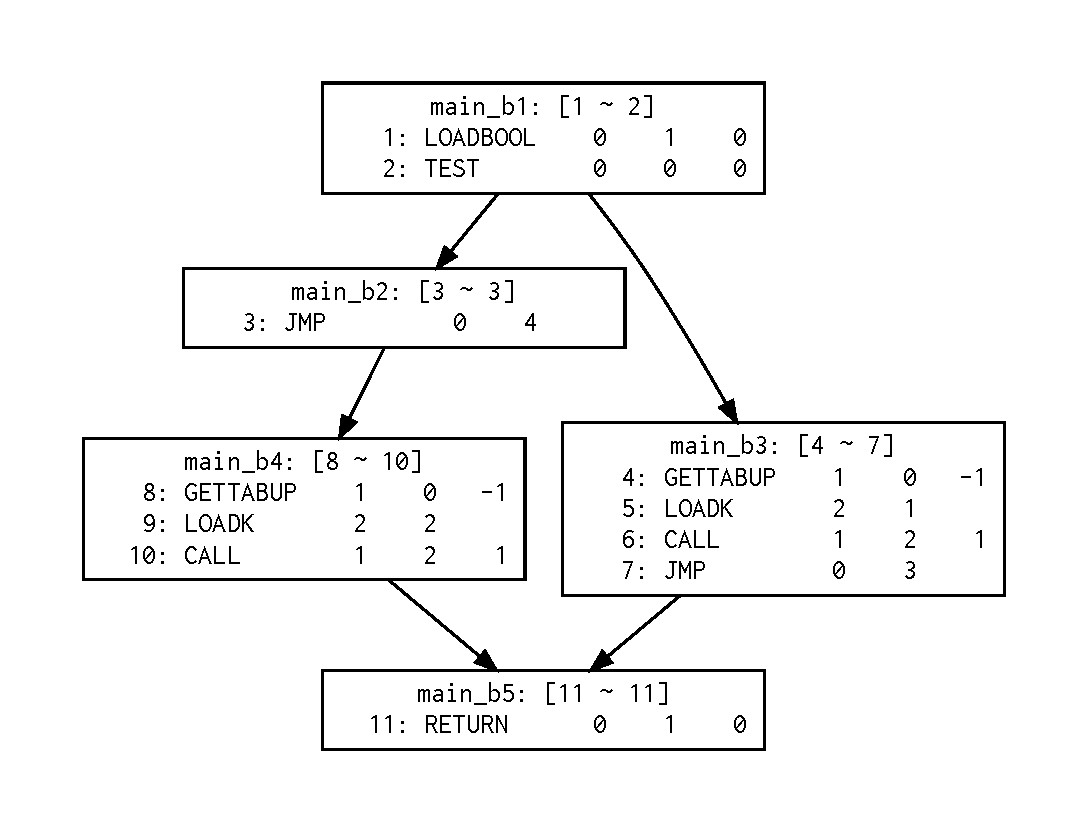
\includegraphics[width=1.3\textwidth]{figure/cfg.pdf}
	\end{figure}
\end{minipage}
\end{frame}
\subsection{optimize}
% \TableOfContents{currentsection}
\begin{frame}
\frametitlesec
以下の最適化を可能な限り何度もおこなう
\begin{itemize}
	\item constant folding (定数畳み込み)
	\item constant propagation (定数伝播)
	\item dead-code elimination (不要式の削除)
	\item function inlining (関数展開)
	\item unreachable block removal (到達不可能なブロックの削除)
	\item unused resources removal (不要資源の削除)
\end{itemize}
\end{frame}

